% created on 2019-12-13
% @author : bmazoyer

%% Lines to compile only this capter
\documentclass[11pt, twoside, a4paper, openright]{report}
\usepackage[utf8]{inputenc}
% \DeclareUnicodeCharacter{223C}{~}

%Bibliography style
% \usepackage[square, numbers]{natbib}
% \usepackage[round]{natbib}
% \usepackage{biblatex}
% \bibliographystyle{unsrtnat}
% \bibliographystyle{unsrt}
% \bibliographystyle{plain}
% \bibliographystyle{aa}
% \usepackage[backend=bibtex,style=authoryear,natbib=true]{biblatex} 
\usepackage[
backend=biber,
style=authoryear,
citestyle=authoryear,
url=false
]{biblatex}
\addbibresource{../source/library.bib}

\usepackage[T1]{fontenc}
\usepackage[french]{babel}
\usepackage{csquotes}  % used for citations (recommended when using biblatex)
%\usepackage{helvet}
%\renewcommand{\familydefault}{\sfdefault}
\usepackage{mathptmx}
\usepackage{amssymb}
\usepackage{geometry} 
\usepackage{xcolor}
\usepackage[absolute,overlay]{textpos}
\usepackage{graphicx}
\usepackage{lipsum}
\usepackage[explicit]{titlesec}
\usepackage{lmodern}
\usepackage{color}
\usepackage{array}
\usepackage{mathtools}
\usepackage{caption}
\usepackage{multicol}
\usepackage{booktabs}
\usepackage{enumitem}
\usepackage{hyperref}
\usepackage{afterpage}
\usepackage{emptypage}
\usepackage{setspace}
\usepackage{pgffor}
    \setlength{\columnseprule}{0pt}
    \setlength\columnsep{10pt}
\usepackage[francais,nohints]{minitoc}
    \setcounter{minitocdepth}{3}
 
 %https://la-bibliotex.fr/2019/02/03/ecrire-les-nombres-et-les-unites-avec-latex/   
\usepackage{siunitx}
% \sisetup{
%     detect-all,
%      output-decimal-marker={,},
%      group-minimum-digits = 3,
%      group-separator={~},
%      number-unit-separator={~},
%      inter-unit-product={~},
%      list-separator = {, },
%      list-final-separator = { et },
%      range-phrase = --,
%      separate-uncertainty = true,
%      multi-part-units = single,
%      list-units = single,
%      range-units = single
%     }
\usepackage{physics}
\usepackage{isotope}

\usepackage[perpage]{footmisc} % to reset the counter of footnote each page

    
\usepackage{fancyhdr}			% Entête et pieds de page. Doit être placé APRES geometry
\pagestyle{fancy}		% Indique que le style de la page sera justement fancy
%\lfoot[\thepage]{} 		% gauche du pied de page
%\cfoot{} 			% milieu du pied de page
%\rfoot[]{\thepage} 
\fancyfoot{} % vide le pied~de~page
\fancyfoot[LE,RO]{\thepage}
\fancyfoot[LO,CE]{}% droite du pied de page
\fancyhead{}	
\fancyhead[LE]{\leftmark}	
\fancyhead[RO]{\rightmark}

\fancypagestyle{plain}{%
\fancyhf{} % vide l’en-tête et le pied~de~page.
\fancyfoot[LE,RO]{\thepage} % numéro de la page en cours en gras% et centré en pied~de~page.
\renewcommand{\headrulewidth}{0pt}
\renewcommand{\footrulewidth}{0pt}}



% Premiere page des chapitres
\newlength\chapnumb
\setlength\chapnumb{3cm}
 
\titleformat{\chapter}[block] {
  \normalfont}{}{0pt} { %police
    \parbox[b]{\chapnumb}{
      \fontsize{120}{110}\selectfont\thechapter} %taille du chiffre
      \parbox[b]{\dimexpr\textwidth-\chapnumb\relax}{
        \raggedleft 
        \hfill{\bfseries\Huge#1}\\ %taille du titre
        \rule{\dimexpr\textwidth-\chapnumb\relax}{0.4pt} %ligne de separation
  }
}
 
 %premiere page chapitre non numerote (remerciement, table des matieres ...)
 
\titleformat{name=\chapter,numberless}[block]
{\normalfont}{}{0pt}
{   
    \parbox[b]{\dimexpr\textwidth}{%   
    \hfill{\bfseries\Huge#1}\\
  \rule{\dimexpr\textwidth}{0.4pt}}}
    
 %   \titleformat{name=\chapter,numberless}[block]
%{\normalfont}{}{0pt}
%{\parbox[b]{\chapnumb}{%
%   \mbox{}}%
%  \parbox[b]{\dimexpr\textwidth-\chapnumb\relax}{%
%    \raggedleft%
%    \hfill{\bfseries\Huge#1}\\
%    \rule{\dimexpr\textwidth-\chapnumb\relax}{0.4pt}}}


%%%    SIunitx
\sisetup{locale = FR,
  % inter-unit-product=\ensuremath{\cdot},
  inter-unit-product=\ensuremath{\,},
  per-mode=reciprocal,
  separate-uncertainty = true,
  detect-all
}
\DeclareSIUnit{\Mpc}{Mpc}
\DeclareSIUnit{\kpc}{kpc}
\DeclareSIUnit{\Gpc}{Gpc}
\DeclareSIUnit{\h}{\textit{h}~}
\DeclareSIUnit{\perh}{\textit{h}^{-1}\,}

%%% Geometry
\geometry{
left=20mm,
top=30mm,
right=20mm,
bottom=30mm
}

%%% Color
\definecolor{bordeau}{rgb}{0.3515625,0,0.234375}

%%% Commands
\newcommand{\Nmocks}{\num{30}}
\newcommand{\hMpc}{h^{-1}\,\mathrm{Mpc}}
\newcommand{\hGpc}{h^{-1}\,\mathrm{Gpc}}
\newcommand{\kms}{\mathrm{km\,s^{-1}}}

\newcommand{\lya}{Ly$\alpha$}
\newcommand{\lyb}{Ly$\beta$}
\newcommand{\lyalya}{Ly$\alpha$(Ly$\alpha$)}
\newcommand{\lyalyb}{Ly$\alpha$(Ly$\beta$)}

\newcommand{\lrf}{\lambda_{\rm RF}}
\newcommand{\kpar}{k_{\parallel}}
\newcommand{\apar}{\alpha_{\parallel}}
\newcommand{\rpar}{r_{\parallel}}
\newcommand{\aperp}{\alpha_{\perp}}
\newcommand{\rperp}{r_{\perp}}
\newcommand{\kperp}{k_{\perp}}

\newcommand{\blya}{b_{\rm Ly\alpha}}
\newcommand{\betalya}{\beta_{\rm Ly\alpha}}
\newcommand{\blyb}{b_{\rm Ly\alpha}}
\newcommand{\betalyb}{\beta_{\rm Ly\beta}}
\newcommand{\dlya}{d_{\rm Ly\alpha}}
\newcommand{\bhcd}{b_{\rm HCD}}
\newcommand{\betahcd}{\beta_{\rm HCD}}
\newcommand{\Fhcd}{F_{\rm HCD}}
\newcommand{\Lhcd}{L_{\rm HCD}}

\newcommand{\imin}{i_{\rm min}}
\newcommand{\imax}{i_{\rm max}}
\newcommand{\jmin}{j_{\rm min}}
\newcommand{\jmax}{j_{\rm max}}

\newcommand{\xioned}{\xi_{\rm 1d}}
\newcommand{\DHub}{D_{H}}
\newcommand{\DM}{D_{M}}

\newcommand{\omegam}{\Omega_M}
\newcommand{\omegac}{\Omega_C}
\newcommand{\omegab}{\Omega_B}
\newcommand{\omegan}{\Omega_\nu}
\newcommand{\omegal}{\Omega_\Lambda}
\newcommand{\omegak}{\Omega_k}
\newcommand{\orad}{\Omega_R}
\newcommand{\ogam}{\Omega_\gamma}
\newcommand{\lcdm}{$\Lambda$CDM}

\newcommand{\picca}{\texttt{picca}}

%%% Rem's command
\newcommand\blankpage{%
    \null
    \thispagestyle{empty}%
    \addtocounter{page}{-1}%
    \newpage}
  
% Command to set up a particular alignment for a cell in tabular :
% \myalign{c}{foo} for instance
\newcommand*{\myalign}[2]{\multicolumn{1}{#1}{#2}}
 
\renewcommand{\thesection}{\arabic{section}}

% Romain
\newcommand{\cRM}[1]{\MakeUppercase{\romannumeral #1}}	% Capital
\newcommand{\cRm}[1]{\textsc{\romannumeral #1}}	% Petit majuscule
\newcommand{\crm}[1]{\romannumeral #1}
% Siècle %
\newcommand{\siecle}[1]{\cRm{#1}\textsuperscript{e}~siècle}



% Thesis title
\newcommand{\PhDTitle}{Les forêts \lya{} du relevé eBOSS : comprendre les fonctions de corrélation et les systématiques} 

% Name
\newcommand{\PhDname}{Thomas Etourneau} 

% Change this variable if you add or remove chapters
\newcommand*{\NumOfChapters}{6}

% Change this variable if you add or remove appendices
\newcommand*{\NumOfAppendices}{2}

% PDF metadata
\hypersetup{
	pdfauthor={\PhDname},
	pdfsubject={Manuscrit de thèse de doctorat},
	pdftitle={\PhDTitle}
}


\begin{document}
%%

\graphicspath{ {../figures/donnees/} }

\chapter{Présentation des données}
\minitoc
\newpage
\thispagestyle{fancy}

Dans le chapitre précédent, nous présentions l'instrument SDSS et sa prise de données qui constitue le relevé eBOSS. Nous présentons ici, comment des photons acquis avec les CCD, les spectres sont déduits, puis comment du spectre de chaque quasar, nous construisons le champ d'absortion.

\section{Réduction des données}
L'observation de chaque plaque fournit des données en deux dimensions : la première correspond aux différentes longueurs d'onde, la seconde aux différentes fibres. La chaîne de réduction des données transforme ces informations en une liste de spectres.
Premièrement, chaque spectre est extrait de l'image acquise par le CCD. Le spectre est étalonné en longueur d'onde à l'aide de lampes à arc. Le flux est calibré en utilisant les spectres des fibres dédiées aux étoiles standards. Puis, le fond du ciel est estimé dans chaque demi plaque grâce aux fibres dédiées, et soustrait à chaque spectre.
La variance dans chaque pixel est ensuite estimée. Elle prend en compte le bruit de photon, le bruit de l'électronique, et aussi les éventuels défauts que présentent les CCD. Les pixels affectés par des rayons cosmiques sont rejetés.
Enfin, pour chaque objet, toutes les expositions sont ajoutées pour former un seul et même spectre, avec un plus grand rapport signal sur bruit. Le nombre typique d'expositions par objet varie entre 4 et 6.

\paragraph{}
Les données que nous utilisons dans ce manuscript sont rendus publiques lors de la seixième publication de données SDSS (DR16\footnote{https://www.sdss.org/dr16/}). Elles sont décrites dans~\cite{Ahumada2019}.

\section{Le catalogue de quasar}
Une fois les spectres extraits, il est important de les classifier afin de construire des catalogues utilisables par les différentes analyses. Pour ce faire, chaque spectre est traité par la chaîne d'identification de SDSS, décrite dans~\cite{Bolton2012}. A chaque spectre est ajusté plusieurs modèles d'étoiles, de galaxies et de quasars. Les modèles sont construits en utilisant les \emph{PCA templates} : des spectres typiques qui sont combinés afin d'ajuster au mieux le spectre à classifier. Une fois tous les modèles ajustés, ils sont triés selon leur $\chi^{2}$ réduit. Le spectre est alors classifié selon le modèle possédant le plus faible $\chi^{2}$ réduit.
Tous les spectres mesurés par SDSS et classifiés comme quasar constituent l'échantillon \emph{superset}. Il contient \num{1440627} objets.

Les quasars, à cause des absorptions intenses comme les DLA ou les BAL\footnote{Les BAL (Broad Absorption Line) sont des quasars qui présentent des absorptions intenses au voisinage de leurs raies d'émission. Cette absorption est interprétée comme étant due à un absorbeur dense situé juste devant le quasar.}, peuvent être difficiles à classifier.
Lors de BOSS, tous les quasars ont été inspectés visuellement (\cite{Paris2016}) afin de confirmer la classification, et d'estimer leur redshifts. Cet échantillon représente \num{297301} objets.
\begin{figure}
  \centering
  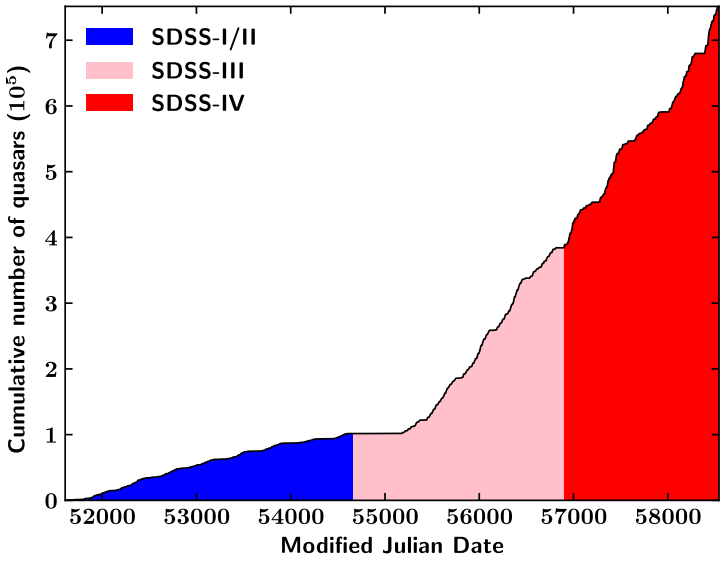
\includegraphics[scale=0.35]{quasar_number}
  \caption{Evolution du nombre de quasars observés par les différentes générations de SDSS en fonction du temps. Les générations SDSS I et II correspondent à $MJD < 54663$ (bleu), SDSS III à $54663 \leq MJD < 56898$ (rose) et SDSS IV à $56898 < MJD < 58543$ (rouge). Crédits : \#prov Lyke in prep}
  \label{fig:quasar_number}
\end{figure}
Cependant, à cause du grand nombre de quasars observés par eBOSS (voir figure~\ref{fig:quasar_number}), l'observation visuelle n'a pas pu être effectuée pour tous ces objets. Une seconde classification, fondée sur la précédente, est alors appliquée~\cite{CITE:Lyke in prep}. Elle est complétée par l'algorithme \texttt{QuasarNET} (\cite{Busca2018}) afin de réduire le nombre d'inspection visuelle à \SI{0.6}{\percent} des spectres, soit \num{8581} spectres. Une sous-échantillon du superset est alors construit. Il contient \num{750426} objets, confirmés comme quasar par la chaîne de traitement précédente.

Pour chaque objet, le catalogue fournit plusieurs estimations de redshift. La chaîne de classification SDSS produit une première estimation. L'algorithme \texttt{QuasarNET} en fournit une seconde. Les spectres inspectés visuellement possèdent une autre estimation. Enfin, l'algorithme \texttt{redvsblue}\footnote{https://github.com/londumas/redvsblue} produit plusieurs estimations de redshift, parmi lesquelles figure \texttt{Z\_PCA} et \texttt{Z\_LYAWG}.

Différents algorithmes sont alors appliqués au catalogue, afin d'identifier les DLA et les BAL présents. L'identification, qui prend place sur les spectres, utilise les différentes expositions additionnées pour chaque objet.
Concernant les DLA, l'algorithme de déctection est décrit dans~\cite{Parks2017}. Il est appliqué sur les quasars à un redshift $2 \leq \texttt{Z\_PCA} \leq 6$, afin d'avoir suffisamment de pixel dans la zone $900 < \lambda_{RF} < \SI{1346}{\angstrom}$. Parmi les \num{270315} spectres inspectés, \num{39514} DLA ont été identifiés, distribués dans \num{35686} spectres.
Concernant les BAL, l'algorithme utilisé est très similaire à celui décrit dans~\cite{Guo2019}. Les BAL sont recherchés dans les spectres ayant un redshift entre \num{1.57} et \num{5.6}. L'algorithme fournit la probabilité qu'un spectre possède un BAL. Le champ \texttt{BAL\_PROB} du catalogue indique cette probabilité.

A la fin, le catalogue ainsi construit (DR16Q dans la suite de ce manuscrit) contient \num{750426} quasars confirmés. Nous référons le lecteur à l'article~\cite{CITE:Lyke in prep} pour davantage d'informations.



\paragraph{}
L'analyse \lya{} finale d'eBOSS (\cite{CITE:dr16}) utilise le catalogue DR16Q. Le redshift des quasars est choisi comme étant \texttt{Z\_LYAWG}. Les quasars sont sélectionnés avec un redshift $1.77 < z \leq 4$. L'échantillon correspondant représente alors \num{341468} objets.


\section{La sélection des forêts}
L'analyse \lya{} finale d'eBOSS, que nous utilisons dans ce manuscrit, utilise l'absorption \lya{} présente dans les spectres de quasars. Les spectres produits par la chaîne de réduction des données SDSS sont rebinnés : 3 pixels du spectre original, d'une taille $\Delta log_{10}(\lambda) \sim 10^{-4}$, sont combinés en 1 seul pixel d'analyse, d'une taille $\Delta log_{10}(\lambda) \sim 3 \times 10^{-4}$. Ceci est fait afin de simplifier la mesure de l'absorption causée par le \lya{}. Dans la suite, l'utilisation de ``pixel'' réfère à ces pixels d'analyse.

L'absorption \lya{} est mesurée dans deux régions disctinctes du spectre. La première, dénommée région \lya{}, correspond aux longueurs d'onde $\num{1040} \leq \lambda_{RF} \leq \SI{1200}{\angstrom}$, c'est à dire entre les raies d'émission \lyb{} et \lya{}. La seconde, dénommée région \lyb{}, correspond aux longueurs d'onde $\num{920} \leq \lambda_{RF} \leq \SI{1020}{\angstrom}$, c'est à dire entre la limite de la série de Lyman et la raie d'émission \lyb{}. Les pixels d'absorption \lya{} dans la région \lya{} sont dénommés pixels \lyalya{}, et ceux dans la région \lyb{} sont dénommés pixels \lyalyb{}.
De plus, l'analyse se limite aux pixels dont la longueur d'onde observée est comprise entre $\num{3000} \leq \lambda_{obs} \leq \SI{6000}{\angstrom}$, à cause notamment des absorptions atmosphériques intenses dans l'UV, et des raies d'émissions du ciel dans le proche infrarouge. Ces limites sur $\lambda_{RF}$ correspondent à un redshift minimal $z_{QSO} = 2$ pour les quasars \lya{}, et $z_{QSO} = 2.53$ pour les quasars \lyb{}. Parmi les \num{341468} quasars utilisés comme traceur (dénommés quasars traceurs), \num{256328} sont utilisés pour leurs absorptions \lya{} dans la région \lya (dénommés quasar \lya{}), et \num{103080} sont utilisés pour leurs absorptions lya{} dans la région \lyb{} (dénommés quasar \lyb{}).

D'autres sélections sont aussi appliquées. Les quasars pour lesquels la probabilité d'avoir un BAL est supérieure à 0.9 sont écartés. Les mauvaises observations durant BOSS ou eBOSS sont mises de côté. De plus, chaque région nécessite au moins 50 pixels. Cette sélection décale le redshift minimal à $z_{QSO} = 2.10$ pour les quasars \lya{}, et à $z = 2.65$ pour les quasars \lyb{}. Enfin, l'ajustement du continu (voir section suivante) échoue pour certains spectres. Ces spectres sont aussi écartés.
Après toutes ces sélections, l'échantillon final contient \num{210005} quasars \lya{} et \num{69656} quasars \lyb{}.
La distribution en redshift des pixels et des quasars traceurs est présentée dans le graphique de gauche de la figure~\ref{fig:pixel_number}.
\begin{figure}
  \centering
  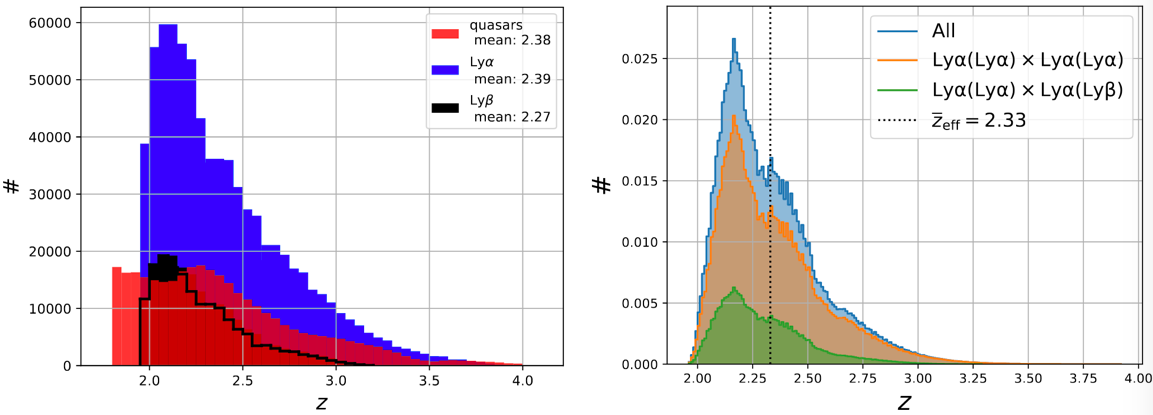
\includegraphics[scale=0.4]{pixel_number}
  \caption{Gauche : distribution en redshift des pixels \lyalya{} (bleu) et des pixels\lyalyb{} (noir) (nombres divisés par 50), ainsi que celle des quasars traceurs (rouge). Droite : \#prov}
  \label{fig:pixel_number}
\end{figure}




\bibliography{../source/library}
\end{document}
